%% Commands for TeXCount
%TC:macro \cite [option:text,text]
%TC:macro \citep [option:text,text]
%TC:macro \citet [option:text,text]
%TC:envir table 0 1
%TC:envir table* 0 1
%TC:envir tabular [ignore] word
%TC:envir displaymath 0 word
%TC:envir math 0 word
%TC:envir comment 0 0
%%
%%
%% The first command in your LaTeX source must be the \documentclass command.
\documentclass[sigconf ,nonacm]{acmart}

%%
%% \BibTeX command to typeset BibTeX logo in the docs
\AtBeginDocument{%
  \providecommand\BibTeX{{%
    \normalfont B\kern-0.5em{\scshape i\kern-0.25em b}\kern-0.8em\TeX}}}


\begin{document}


\title{Music Genre Classification}

\author{Ruochen Kong}
\email{ruochen.kong@emory.edu}
\affiliation{%
  \institution{Emory University}
  \city{Atlanta}
  \state{Georgia}
  \country{USA}
}

%%
%% Keywords. The author(s) should pick words that accurately describe
%% the work being presented. Separate the keywords with commas.
\keywords{Signal Processing, Data Mining, Machine Learning}
\begin{abstract}
Searching music by genre is a function implemented in almost all music apps, so an accurate algorithm to classify the music is required. The existing research papers generally classified music into nearly five genres, but in the real world, much more detailed genres exist. This rough classification may further cause an unsatisfaction of the user experience. In this project, I aim to investigate the signal of the music in 19 genres, extract distinguishable features, and create a classification model. The result may form a more detailed automatic classification model for music.
\end{abstract}

\maketitle

\section{Introduction}
Major music applications, such as Spotify, Apple Music, or Gnoosic, have all allowed users to search by genre. The categorization quality, however, is somewhat unsatisfactory. In order to reduce the number of incorrectly classified music, algorithms in use tend to reduce the number of available genres. As stated by Tamatjita (2016), the more genres to be classified, the lower the accuracy \cite{7930314}. This drawback is understandable because even humans will feel harder to distinguish between more genres, but pursuing a more accurate automatic classification method is still necessary. The goal of this project is to establish a method to classify musics into more genres. Several previous reaserch paper has already developed methods to classify music with a high accuracy, but few of them achieved with more than 10 different genres. In the real world, however, users may choose series of genres in order to find their favorite songs. Then, in this condition, these limited generes can not satisfy. In this project, I will develop the model on a dataset posted on Kaggle \cite{kaggle}. This dataset, labeled with 19 different genres, has 19.9k individuals in the training dataset and 5k in the testing dataset. To develop the model, I will first visualize several music signals in different genres to determine possible features, such as the beat, the volume, or the frequency. I will then base on common classification models, such as CNN or Random Forest, to either improve on them or form an embedded model. Finally, I will evaluate the result with commonly used metrics, including ROC, AUC, F1-score, precision, recall, and accuracy.

\section{Problem Definition}
The music data are stored as {\it .ogg} files which can be converted into a series of frequencies with existed packages. Because the music is binaural, when converting into arrays, they will have a dimension as $(n,2)$ with $n$ represents the number of recorded signals and $2$ represents the left and right channel. 
\begin{figure}
  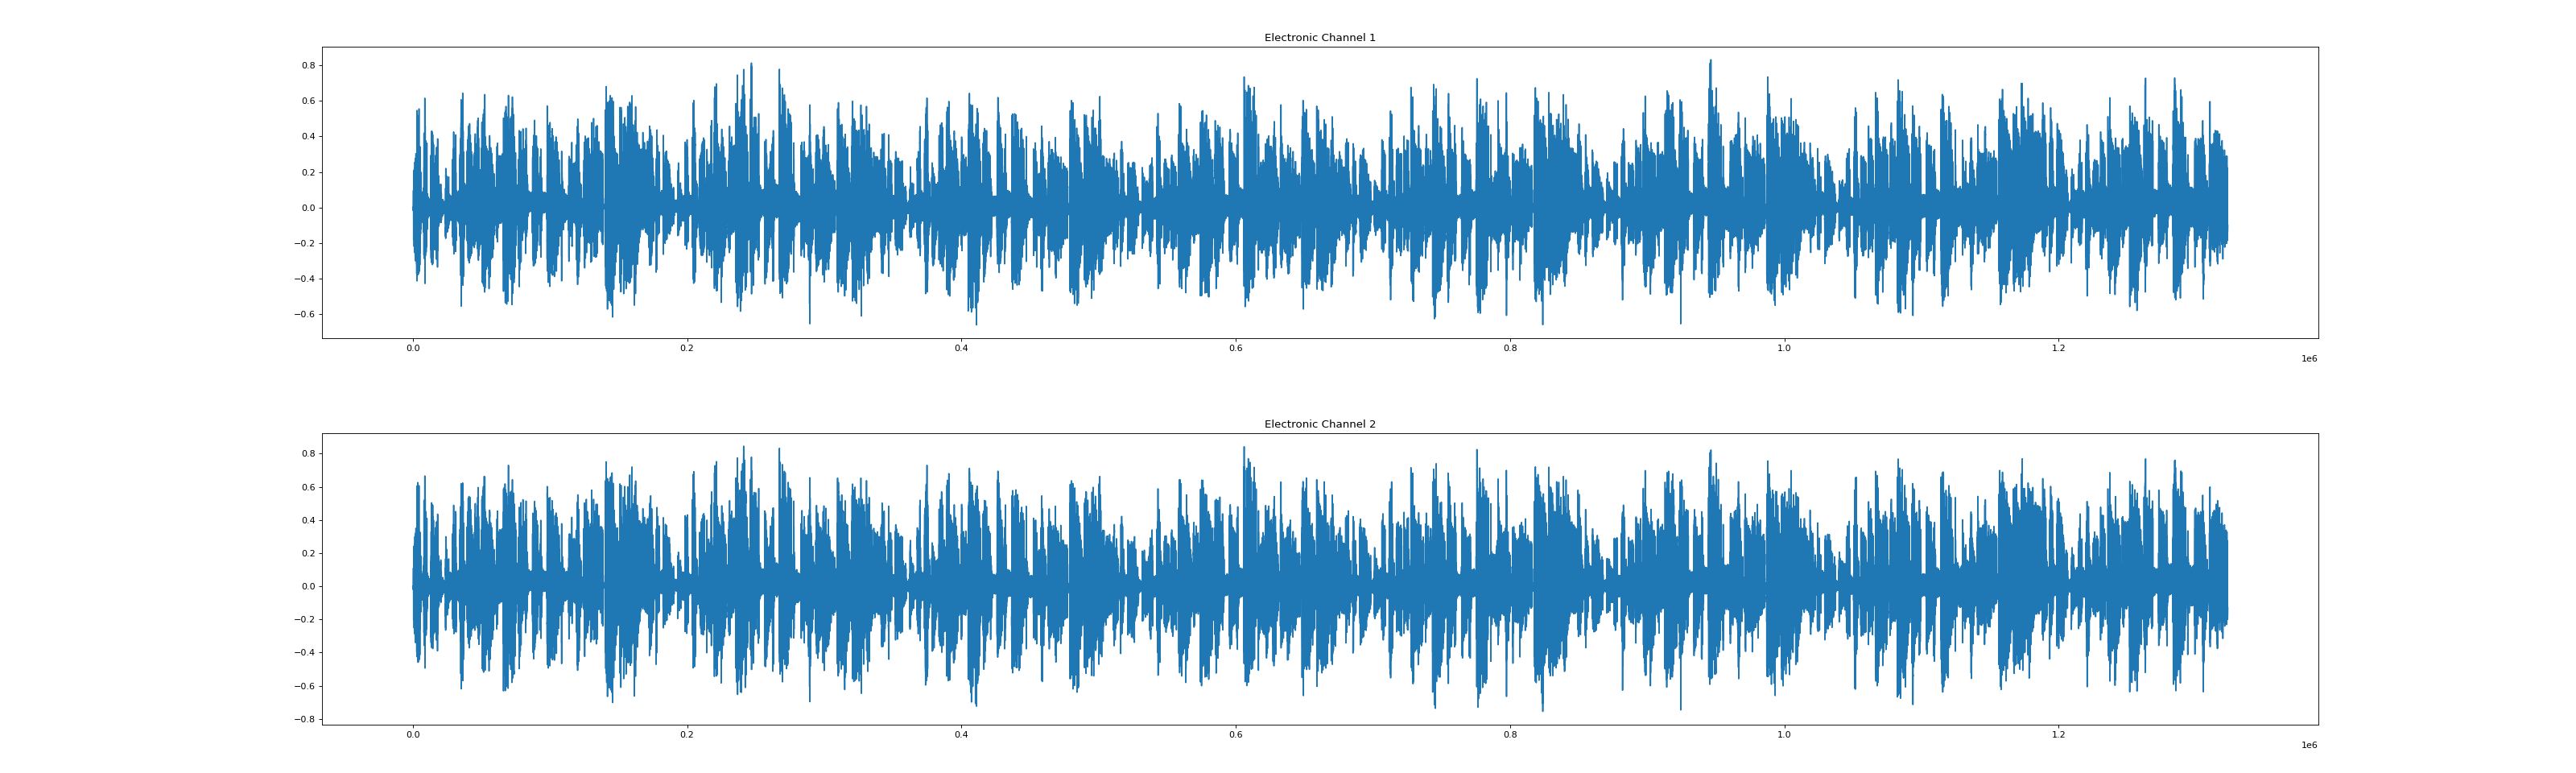
\includegraphics[width=\columnwidth]{Electronic.png}
  \caption{Genre: Electronic}
  \Description{Signals for Electronic Music}
\end{figure}
\begin{figure}
  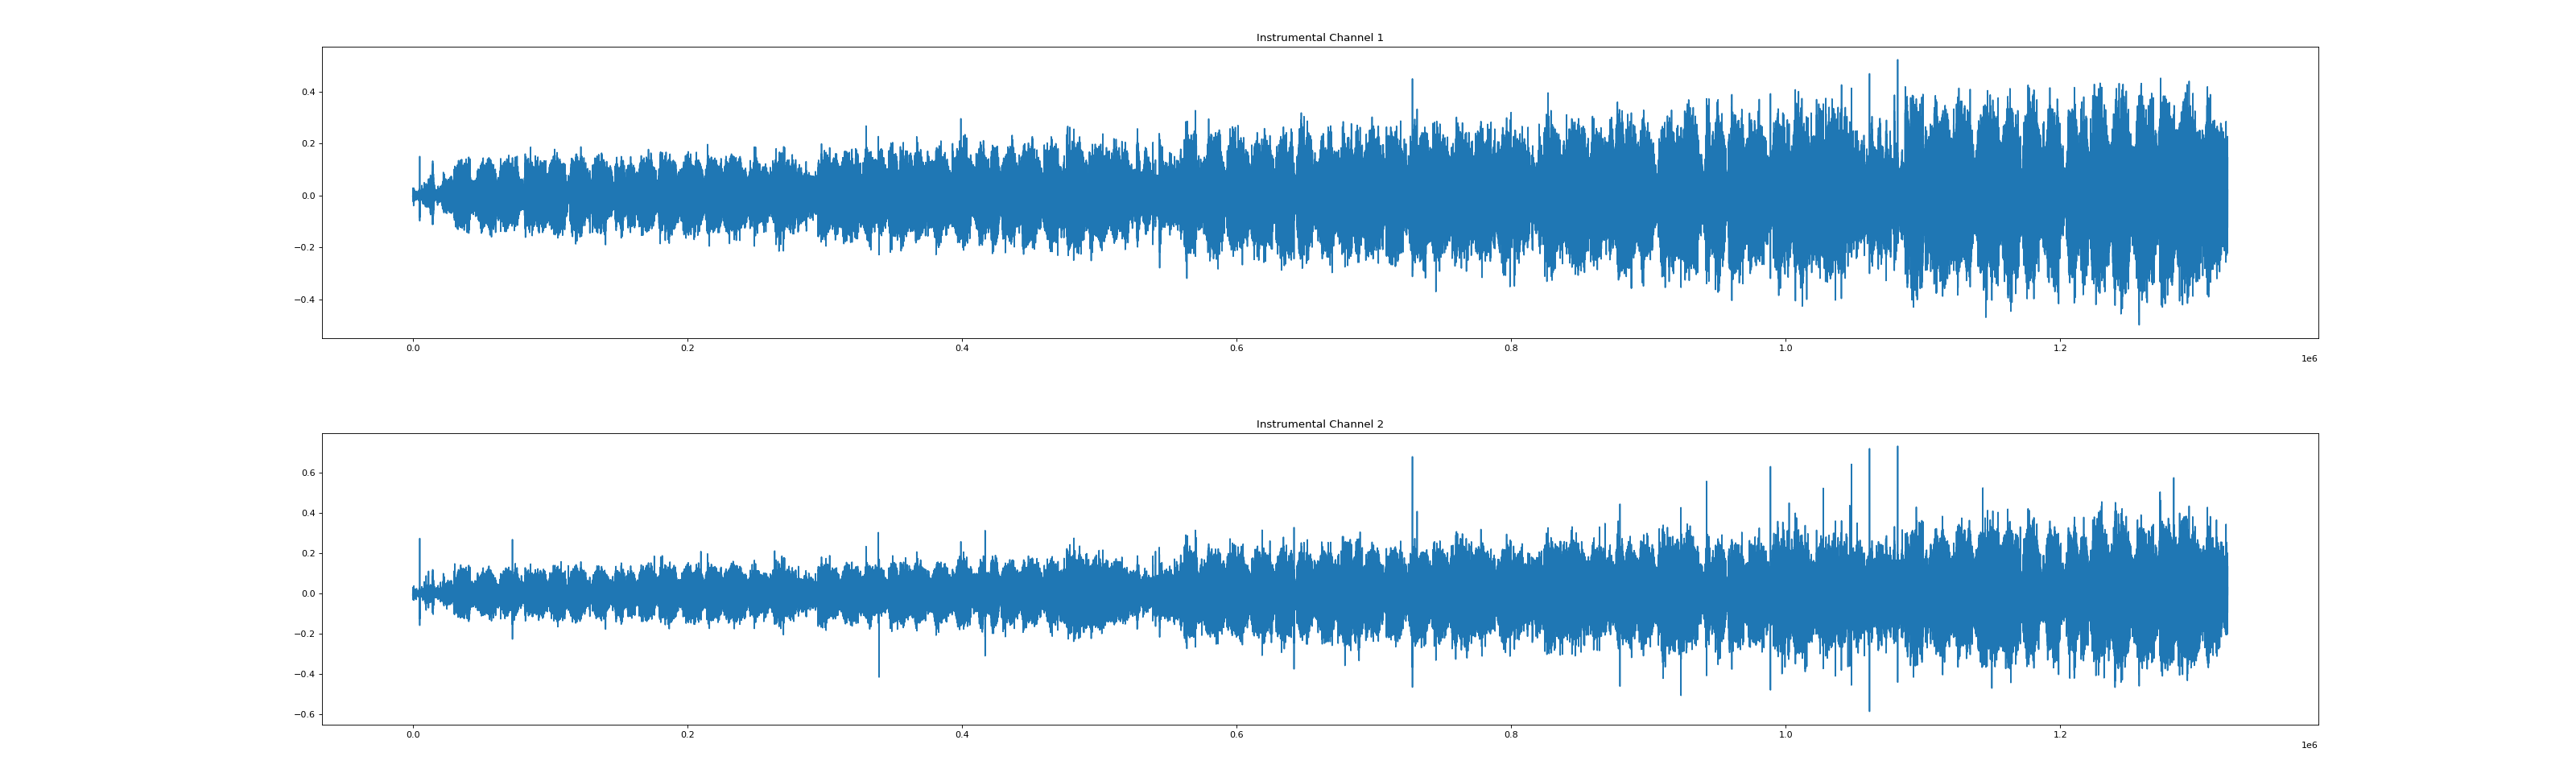
\includegraphics[width=\columnwidth]{Instrumental.png}
  \caption{Genre: Instrumental}
  \Description{Signals for Instrumental Music}
\end{figure}

Figure 1 and 2 represents an example of electronic music and instrumental music. As can be seen from the figures, these two kinds of music tend to diverge significantly on the view of signals. For example, electronic music may have shorter beats, which will be extracted as a feature to be considered. Other possible features will be determinded in further analysis. 

Assume the extracted features are stored as matrix $X \in \mathbb{R}^{n\times p}$ with $n$ represents number of music and $p$ represent number of features, and also denote $y = \{y_i : y_i \in \{0,1,\ldots,18\}\}$, then the goal is to create a model $\mathcal{M}: X \to \hat{y}$ with minimal distance between $y$ and $\hat{y}$. The distance would be a combination of L1-norm and L2-norm.

\section{Materials and Methods}
\subsection{Dataset}
The dataset is separated as $19,922$ training data and $5,078$ testing data. These music files are then transformed into arrays by the {\it soundfile} package in python. The labels are listed in order as electronic, rock, punk, experimental, Hip-Hop, folk, chiptune/glitch, instrumental, pop, international, ambient electronic, classical, old-time/historic, Jazz, country, Soul-RnB, spoken, Blues, and easy listening.
\subsection{Evaluation Metrics}
The most common ones are:
\begin{align*}
ACC &= \frac{TP+TN}{P+N},\ &F_1 &= \frac{2TP}{2TP+FP+FN}\\
precision &= \frac{TP}{TP+FP},\ &recall &= \frac{TP}{P}
\end{align*}
Since this is not a binary classification task, an average value would be used.




\bibliographystyle{ACM-Reference-Format}
\bibliography{ref}
\end{document}